\item \points{2b} {\bf Implement Outer Loop}

In the \texttt{maml.py} file, complete the implementation of the \texttt{MAML.\_outer\_step} which computes the MAML objective (and more metrics). Pay attention to the inline comments and docstrings. \\
\textbf{Hint}: to understand how to use the Boolean \texttt{train} argument of \texttt{MAML.\_outer\_step}, read the documentation for the \texttt{create\_graph} argument of \texttt{autograd.grad}.

Assess your implementation of vanilla MAML on 5-way 1-shot Omniglot. 

You can run the experiment by executing: \texttt{python maml.py}

Comments from the previous part regarding arguments, checkpoints, TensorBoard, resuming training, and testing all apply. Use 1 inner loop step with a \textbf{fixed} inner learning rate of 0.4. Use 15 query examples per class per task. Do not adjust the outer learning rate from its default of $0.001$.

Your plot of the validation post-adaptation query accuracy over the course of training should look like this.
\begin{center}
    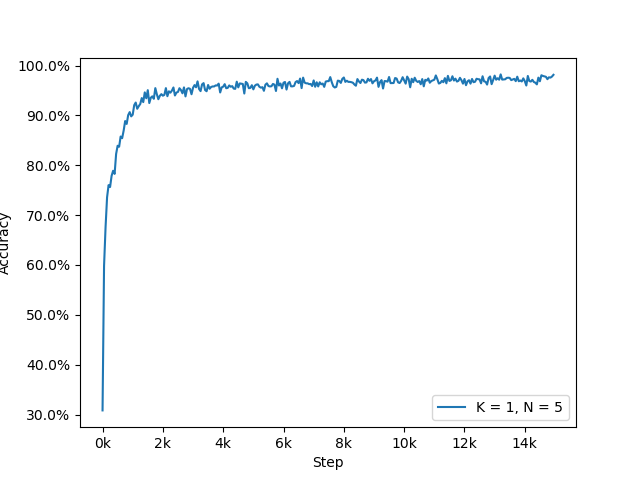
\includegraphics[width=0.75\linewidth]{./figures/maml_q1}
\end{center}

\textbf{Hint}: you should obtain a query accuracy on the validation split of at least $96\%$.

